\section{Spannungsregler/Stromversorgung}\hartl{280}
\subsection{Aufgaben von Spannungsreglern}
\begin{itemize}
  \item Stabilisieren Versorgungsspannung der Elektronik
  \item Lieferung von genügend Strom für Elektronik
  \item Filterung von störenden Frequenzen auf Speisungs-Eingang
\end{itemize}

\subsection{Lineare Spannungsregler}\hartl{280}
Für alle linearen Spannungsregler gilt: \begin{equation}
P_{V}=(V_{E}-V_{a})*I_{a}
\end{equation}\\
Einsatz für geringer Spannungsunterschied zwischen eingangsspannung und der
geregelten Ausgangsspannung

\begin{longtable}{|l|l|l|}
\hline
\begin{minipage}{4cm}
\textbf{Spannungsstabilisierung mit Transistor}\\\hartl{280}
\end{minipage}
&
\begin{minipage}{6cm}
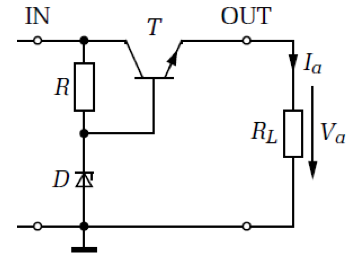
\includegraphics[width=6cm, height =
4cm]{pictures/transistorStabilisierung}
\end{minipage}
&
\begin{minipage}{8cm}
\begin{gather}
I_{E}=I_{L}\approx I_{C}\\
U_{E}=U_{A}+U_{CE}\\
U_{A}=U{Z}-U_{BE}\\
R_{V}=\frac{U_{E}-U_{Z}}{I_{Z}+I_{B}}\\
I_{B}=\frac{I_{C}}{B}\\
R_{i}\approx\frac{r_{Z}}{\beta} 
\end{gather}
\begin{tabular}{ll}
$U_{E}$:&unstab. Eingangsspannung\\
$U_{A}$:&stab. Ausgangsspannung\\
$U_{Z}$:&ZDioden-Spannung\\
$U_{CE}$:&Kollektor-Emitterspannung\\
$U_{BE}$:&Basis-Emitterspannung\\
$I_{Z}$:&Strom durch die Z-Diode\\
$I_{C}$:&Kollektorstrom\\
$I_{B}$:&Basisstrom\\
$B$:&Gleichstromverstärkung\\
$R_{i}$:&Innenwiderstand der Schaltung\\
$r_{Z}$:&dyn. Innenwiderstand der Z-Diode\\
$\beta$:&Stromverstärkungsfaktor des Transistors
\end{tabular}
\end{minipage}
\\
\hline
\begin{minipage}{4cm}
\textbf{Festspannungsregler}\\\hartl{282}
\end{minipage}
&
\begin{minipage}{6cm}
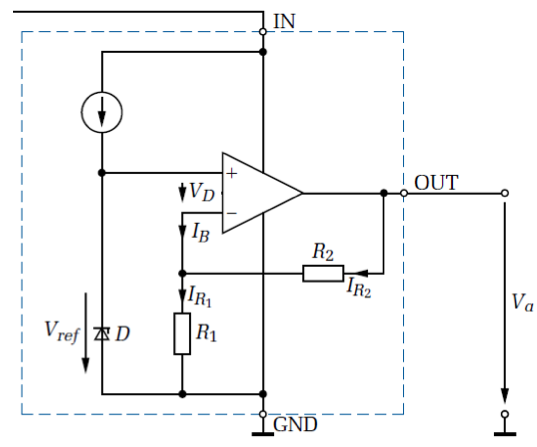
\includegraphics[width=6cm, height =
4cm]{pictures/festStabilisierung}
\end{minipage}
&
\begin{minipage}{8cm}
\begin{gather}
V_{ref}=V_{D}+V_{R1}\\
V_{a}=I*(R_{2}+R_{1})=\frac{V_{ref}}{r}*4R=4*V_{ref}
\end{gather}
\end{minipage}
\\
\hline
\begin{minipage}{4cm}
\textbf{Festspannungsregler mit einstellbarer Ausgangsspannung}\\\hartl{284}
\end{minipage}
&
\begin{minipage}{6cm}
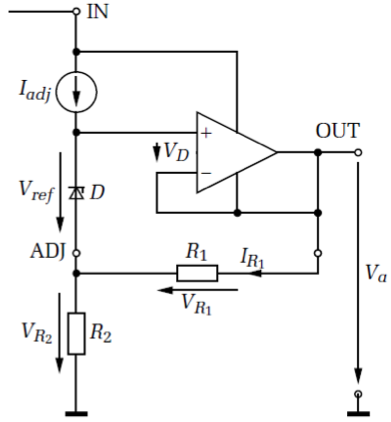
\includegraphics[width=6cm, height =
4cm]{pictures/einstellbarStabilisierung}
\end{minipage}
&
\begin{minipage}{8cm}
\begin{gather}
V_{a}=V_{R1}+V_{R2}=V_{ref}+R_{2}*(I_{R1}+I_{adj})=\notag\\=V_{ref}+R_{2}*(\frac{V_{ref}}{R_{1}}+I_{adj})\\
\text{für }I_{adj}<< I_{R1} \to V_{a}=V_{ref}*(1+\frac{R_{2}}{R_{1}})
\end{gather}
\end{minipage}
\\
\hline
\end{longtable}

\subsection{Schaltregler}\hartl{285}
\begin{longtable}{|l|l|l|}
\hline
\begin{minipage}{4cm}
\textbf{Abwärtswandler (Buck Converter)}\\\hartl{285}
\end{minipage}
&
\begin{minipage}{6cm}
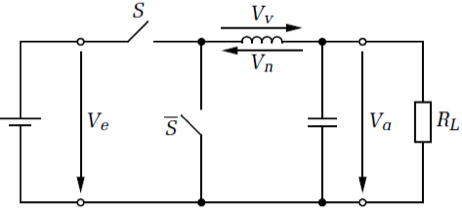
\includegraphics[width=6cm, height =4cm]{pictures/abwaertsWandler}
\end{minipage}
&
\begin{minipage}{8cm}
Es gilt: $0\leq V_{a}\leq V_{e}$\\
\begin{gather}
\text{Son}\notag\\
V_{V}=L*\frac{\Delta I_{L}}{\Delta t}\\
V_{e}=V_{V}+V_{a} \to V_{e}=L*\frac{\Delta I_{L}}{\Delta t}+V_{a}\\
\text{Soff}\notag\\
V_{n}=V_{a}=L*\frac{\Delta I_{L}}{\Delta t}\\
\Delta I_{L}=(V_{e}-V_{a})*\frac{1}{L}*t_{ein}\\
V_{a}=\frac{t_{ein}}{t_{aus}+t_{ein}}*V_{e}=d*V_{e}
\end{gather}
\begin{tabular}{ll}
d:&Tastverhältnis/Duty Factor\\
\end{tabular}
\end{minipage}
\\
\hline


\end{longtable}